\documentclass[a4j,12pt]{jreport}
\usepackage[dvipdfmx]{graphicx}
\usepackage{here}
\title{生物情報実験法2019 岩崎先生}
\author{05-195512 生物情報科学科3年 \\ 山口尚人}
\date{\today}
\begin{document}
\maketitle




\chapter{課題2 微生物ゲノムの解析}

\section{目的}
広大な人類未踏の領域である微生物ゲノムを自由な発想で解析することで、その解析手法を学ぶと共に、新規の発見を目指す。

\section{解析内容}
極限環境微生物のゲノムを比較し、dN/dS解析をおこなった。その微生物に特徴的な極限環境で重要な役割を果たす遺伝子は正の自然選択を受けているという仮説を元に、
その遺伝子を配列から発見することを目指し、2種類の微生物ゲノムを比較し、dS/dN解析をおこなった。
松井先生にお話を伺う中で、強い放射線耐性を持つ微生物に興味を持った。
現在までに見つかっている強い放射線耐性を持つ微生物の多くは、放射線によるゲノムの損傷を予防するのではなく、損傷したゲノムを修復する能力が高いということを知り、この遺伝子の機能やその応用可能性を魅力的に感じた。
特に、よく解析されているDeinococcus Radioduransをはじめとする、Deinococcus属ではその属に特有の、DNAの結びつき二本鎖切断の修復効率をあげるとされるPprAタンパク質の立体構造が決定されている[2]。

高い放射線耐性を持つ微生物は、Deinococcus Radioduransが有名であるが、それ以外にも多く存在しており、
Deinococcus属に属する微生物の他、Ruburobacter Radiotolerans、Kineococcus radiotolerans、Halobacterium salinarum NRC-1などがあげられる。

今回の解析の主な目的は、極限環境微生物の中でも特に、高放射線耐性微生物のゲノムに着目することで、高い放射線耐性をどのように獲得してきたかを発見すること、もしくは、ゲノムの比較によって、放射線耐性に寄与している遺伝子を見つけることができるのではないかという仮説を検証することである。

\section{具体的な手順}
    dN/dS解析の方法、手順に関しては[1]を参考にした。
    \begin{enumerate}
        \item 2種の微生物ゲノムを選択した

        本解析では、2つのゲノムのアノテーションされたゲノム領域を用いた。これらの微生物のコドン表は11番であるが、例外の含まれていたため、各遺伝子の塩基配列だけでなく、アノテーションされた翻訳後のアミノ酸配列も必要であったことから、
        両者ともgenomicのGenbankファイルを用いた。
        \item 2つのゲノムから、オーソログを抽出
        
        [1]で紹介されているように、複数の方法が考えられる。代表的なものは、BLASTをRBB(Reciprocal Best BLAST hit) methodである。
        それ以外には、OMA (Orthologous MAtrix)やOrthoMCLといったオーソログ推定データベースがあげられる。
        また、BLASTスコアに関連する遺伝子長の偏りを考慮に入れることによってオルソログの精度を高めたOrthoFinderというソフトウェアも考慮に入れた。
        しかし、今回は、インストールの手間や、APIドキュメントの簡潔さの観点から、OMAを用いることにした。OMAは、REST APIを提供しており、ドキュメントも非常にわかりやすく、適度にアップデートされており、
        すぐに使える上、それなりに信頼できると考え、選択した。

        比較したい2つのゲノムのtaxonomy idを取得し、それらをクエリとしてGETリクエストを送ることで、2つのゲノムのオーソログのタンパク質情報を得ることができる。
        それらには各ゲノムでの開始地点、終了地点、またUniProtなどでのユニークなIDなどが含まれる。
        
        \item 各オーソログのアミノ酸配列のアライメントをおこなった
        
        次のステップで後述するように、dN/dS解析にあたってコドンベースのアライメントが必要であり、その前段階としてアミノ酸配列のアライメントが必要である。
        そこで、アライメントツールとしてClustal OMegaを用いた。コドンベースのアライメントをオプションと入力の変更によっておこなえるPRANKも考慮に入れたが、
        Clustal OMegaが使い易かったこと、後述のPAL2NALと組み合わせることでも目的を達成できそうであったため、前者を選択した。

        1つ前のステップで得られたオーソログのアミノ酸配列を入力として、アライメントをおこなった。

        \item 各オーソログに対してコドンベースのアライメントをおこなった
        
        次のステップは各オーソログの塩基配列をアライメントすることであるが、当然オーソログ同士の配列長は異なることが多い。また、今回の解析の目的は、非同義置換、同義置換の比を求めることであるから、
        各アミノ酸に対応するコドンの関係がアライメントによってずれてしまう(フレームシフト)と、正しいdN/dS値を算出することができない。
        そこで、dN/dS解析にあたっては、コドンベースでの塩基配列のアライメントをおこなう必要がある。これはタンパク質のアミノ酸配列同士をアライメントし、その後それに対応するコドンを元の塩基配列を参照しながら
        塩基配列をアライメントする方法である。これによってコドンの対応が崩れることなく、非同義置換、同義置換の解析をおこなうことができる。
        
        そこで、今回は、このコドンベースのアライメントをおこなうソフトウェアである、PAL2NALを用いた。
        これはperlスクリプトであり、Web上からローカルにdownloadすることで、jupyter notebookからコマンドライン実行で実行できたため、利用した。
        PAL2NALは2019年現在、2011年から更新されていないようであった。このコドンベースのアライメントはさほど複雑ではないと考えられるので自分でプログラムを書くこともできたとは思うが、
        時間の関係上、このソフトウェアを信頼し利用した。
        
        PAL2NALに対する入力は、OMAのREST APIから得られたオーソログのタンパク質のアミノ酸配列と、その各ゲノム上での位置を利用してGenbankのゲノムデータ上から取得した、対応する遺伝子領域の塩基配列である。(これを2セット用意した)

        \item アライメントされた塩基配列を入力とし、dN/dSの値を算出した
        
        dN/dS値の算出では、PAML(Phylogenetic Analysis by Maximum Likelihood) に含まれるCodeMLを用いた。
        アライメントされた塩基配列と比較するゲノムの系統関係を元に、非同義置換、同義置換の数、率、それらの比率を算出するプログラムである。
        CodeMLは、枝モデル (branch models), サイトモデル (site models), 枝サイトモデル (branch-site models) の 3 種類モデルに基づいた解析が可能である。

        枝モデルは,遺伝子系統樹のある枝で正の自然選択が働いたかどうかを検定する解析モデルであり[3]、今回のような、2種類のみのゲノムのペアワイズの比較には不適当であると考え、
        サイトモデルは、枝間の $\omega$ を変化させず,サイト間での $\omega$ の変異を検定するモデルである[3]。

    \end{enumerate}



\section{結果}
以下に、Deinococcus Radiodurans R1とThermus Thermophilus HBの85個のオーソログ遺伝子について、dN/dSの値を算出し、
プロットした結果を示した。

    
\begin{figure}[H]
    \begin{center}
      \begin{tabular}{cc}
        % 1
        \begin{minipage}{0.5\hsize}
          \begin{center}
            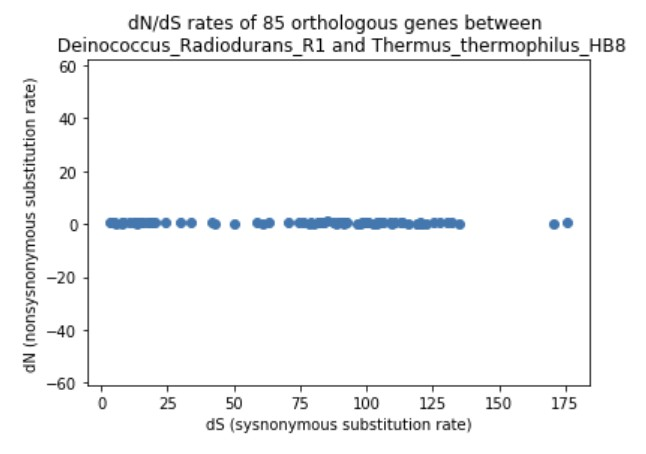
\includegraphics[width=\hsize]{images/result1.jpg}
            \caption{Deinococcus RadioduransとThermus Thermophilusの85個のオーソログ遺伝子のdN/dSを1:1スケールでプロットしたもの}
          \end{center}
        \end{minipage}
  
        % 2
        \begin{minipage}{0.5\hsize}
          \begin{center}
            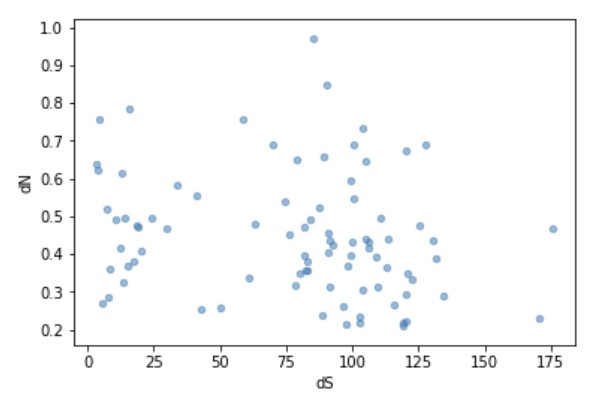
\includegraphics[width=\hsize]{images/result2.jpg}
            \caption{Deinococcus RadioduransとThermus Thermophilusの85個のオーソログ遺伝子のdN/dSのプロットを拡大したもの}
          \end{center}
        \end{minipage}
  
      \end{tabular}
    \end{center}
  \end{figure}

  \begin{figure}[H]
    \begin{center}
      \begin{tabular}{cc}
        % 1
        \begin{minipage}{0.5\hsize}
          \begin{center}
            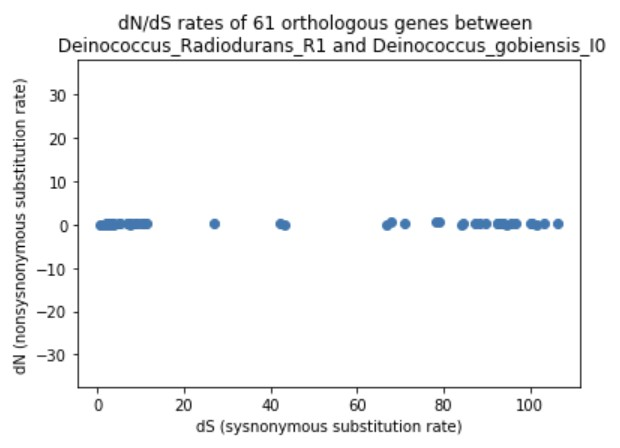
\includegraphics[width=\hsize]{images/result3.jpg}
            \caption{Deinococcus RadioduransとDeinococcus Gobiensisの61個のオーソログ遺伝子のdN/dSを1:1スケールでプロットしたもの}
          \end{center}
        \end{minipage}
  
        % 2
        \begin{minipage}{0.5\hsize}
          \begin{center}
            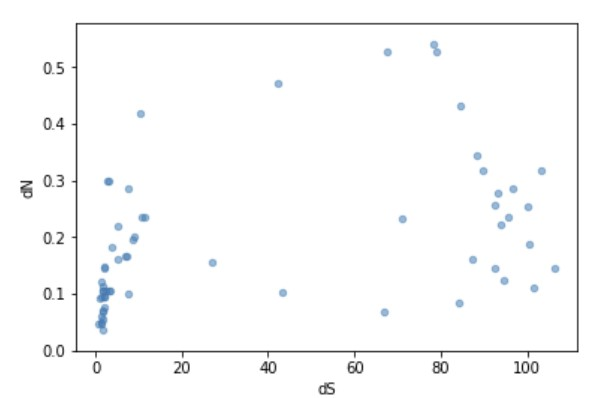
\includegraphics[width=\hsize]{images/result4.jpg}
            \caption{Deinococcus RadioduransとDeinococcus Gobiensisの61個のオーソログ遺伝子のdN/dSのプロットを拡大したもの}
          \end{center}
        \end{minipage}
  
      \end{tabular}
    \end{center}
  \end{figure}

また、同様のプログラムを用いて、Deinococcus Radiodurans R1とDeinococcus Gobiensis I0の個のオーソログ遺伝子についても、dN/dSの値を算出し、プロットした結果を示した。

圧縮して提出したプログラムファイル、入出力ファイルは、GitHubにもアップロードされている。[https://github.com/Naoto-Yamaguchi/3s-iwasaki-kadai2]



\section{考察}
結果の図のどちらを見てもわかるように、各オーソログ遺伝子のdN/dSの値は、0.01よりも小さいものがほとんどであり、dN/dSは1以下であるばかりか、同義置換率が非同義置換率に比べて
非常に大きい値を取っているということがわかった。
また、同義置換率が桁違いに大きいものが多数ある。
これにはいくつかの理由が考えられる。
  \begin{enumerate}
    \item オーソログの抽出によるもの
    
    OMAデータベースから抽出されてオーソログは、種間での保存度合いが高いもののみに偏っていた可能性が考えられる。
    \item 比較する2種類のゲノムがdN/dS解析に適していない
    
    今回、Deinococcus Radioduransにまず着目し、その種と進化的に近く、かつ放射線耐性がそこまで高くないThermus Thermophilusとの比較をおこなった。
    また、その結果からより近い種での解析も試そうと考え、Deinococcus Gobiensisとの比較もおこなった。
    しかし、この比較対象の検討が十分であったとは言えず、また目的を達成するために相応しいものではなかった可能性もあり、再検討が必要である。
  
    \item 正しい解析がおこなえていなかった
    
    CodeMLのモデル選択が適切でなかった

  \end{enumerate}



\section{利用したデータ}
    \begin{itemize}     
        \item Deinococcus Radiodurans R1
        
        RefSeqデータ 
        \item Thermus Thermophilus HB
        
        RefSeqデータ
        \item Deinococcus Gobiensis I0
        
        アノテーションされたGenBankファイル

    \end{itemize}


\section{参考文献}
  [1] Daniel C.Jeffares et all.(2015)「A Beginners Guide to Estimating the Non-synonymous to Synonymous Rate Ratio of all Protein-Coding Genes in a Genome」

  [2] M.Adachi (2019) 「Extended Structure of Pleiotropic DNA Repair-Promoting Protein PprA from Deinococcus radiodurans」

  [3] Ziheng Yang(2017)「PAML Manual User Guide」
  
\end{document}